%%%%%%%%%%%%%%%%%%%%%%%%%%%%%%%%%%%%%%
%%%%%%%%%%%%%%%%%%%%%%%%%%%%%%%%%%%%%%
% Do not edit the TeX file your work
% will be overwritten.  Edit the RnW
% file instead.
%%%%%%%%%%%%%%%%%%%%%%%%%%%%%%%%%%%%%%
%%%%%%%%%%%%%%%%%%%%%%%%%%%%%%%%%%%%%%




On the Iris data, we evaluated the expected number of clusters for a range of
$\alpha$ between 0.5 and 15. Then we chose three $\alpha_0$ values, 3, 8, and
13, and constructed the linear approximation centered at each of these
$\alpha_0$s.
% The linear approximation did quite well for choices of $\alpha$
% close to $\alpha_0$, as seen in \prettyref{fig:parametric_sens_plot}.
We note that the linear approximation is more accurate when extrapolating from
more clusters to fewer clusters, as can be seen from the fact that the linear
approximation in the rightmost panel of \prettyref{fig:parametric_sens_plot} is
accurate across the entire range of $\alpha$, whereas the leftmost panel is not.


\begin{knitrout}
\definecolor{shadecolor}{rgb}{0.969, 0.969, 0.969}\color{fgcolor}\begin{figure}[!h]

{\centering 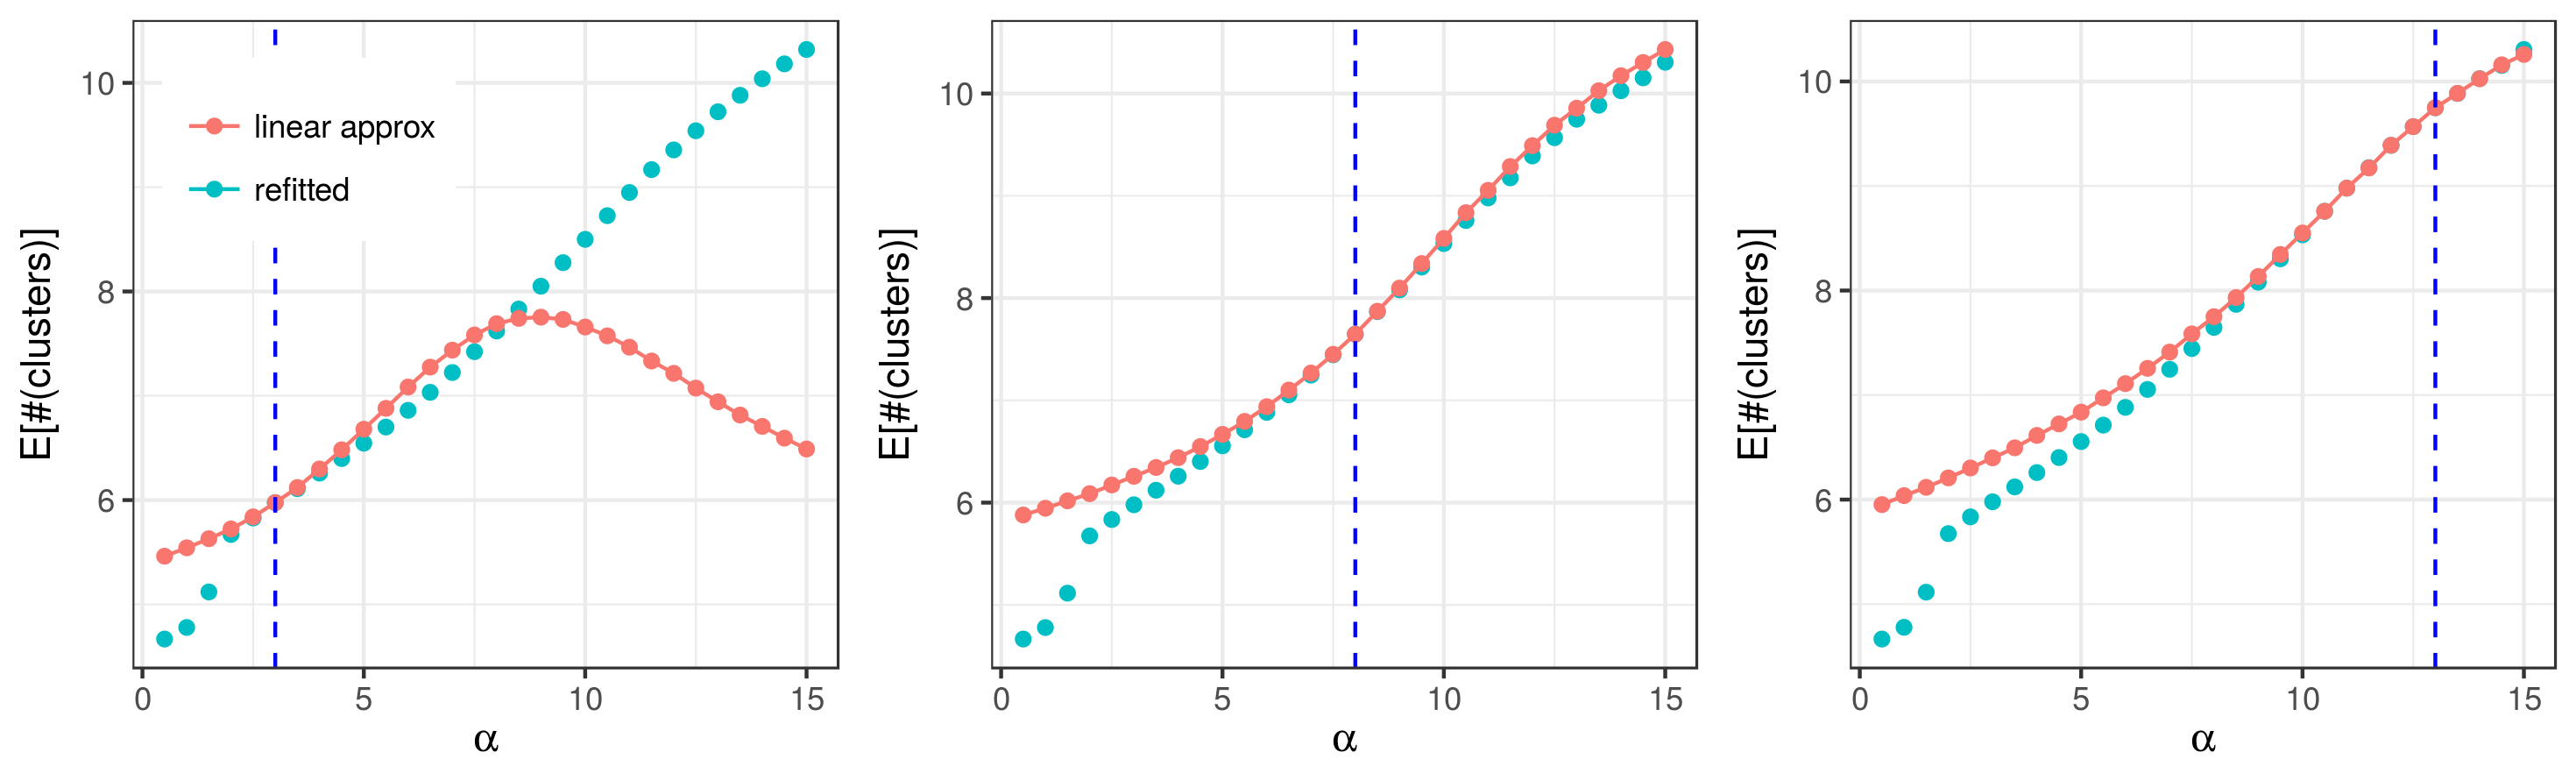
\includegraphics[width=0.98\linewidth,height=0.294\linewidth]{figure/parametric_sens_plot-1} 

}

\caption[Comparison of the expected number of clusters computed by re-optimizing versus the linear approximation]{Comparison of the expected number of clusters computed by re-optimizing versus the linear approximation.  The blue vertical line indicates the location of $\alpha_0$.}\label{fig:parametric_sens_plot}
\end{figure}


\end{knitrout}
